\documentclass[10pt, a4paper, oneside, twocolumn]{article}

% encoding and language
\usepackage[utf8]{inputenc}
\usepackage[T1]{fontenc}
\usepackage[english]{babel}
\usepackage[babel]{csquotes}

% math packages
\usepackage{amsmath}
\usepackage{amsthm}
\usepackage{mathrsfs}
\usepackage{amssymb}

% graphics support
\usepackage{graphicx}
\usepackage{epsfig}
\usepackage{float}
\usepackage{color}

% nice tables
\usepackage{booktabs}

% hyperrefs
\usepackage{hyperref}

% metadata
\title{Bioinformatics Practicum\\\textbf{Project 5 - Phase Diagram of a Noble Gas}}
\author{Sebastian Hewett - Stephan Weißbach - Max Riedl - Laksan Nathan}
\date{\today}

\begin{document}
\maketitle

\section{Introduction to Molecular Dynamics Simulations}

Molecular dynamics (MD) is a computer simulation method for studying atoms and molecules in motion ~\cite{Gonzalez}. Following the laws of classical mechanics, i.e. numerically solving Newton's 2nd law (\ref{eq:2nd law}), MD simulations allow insights into trajectories for each atom \(i\) in a system constituted by \(N\) atoms. Forces between the particles and their potential energies are calculated using force fields.
%  this commented blank line prevents start of a new paragraph
\begin{equation}\label{eq:2nd law}
F_i = m_i a_i.
\end{equation} %  this commented blank line prevents start of a new paragraph
Here, \(m_i\) is the atom mass, \(a_i = \frac{d^{2}r_i}{d^{2}t}\) its acceleration, and \(F_i\) the force acting upon it, due to the interactions with other atoms.

Since molecular systems typically consist of a large number of particles, it is impossible to analytically determine the properties of such complex systems; MD simulation avoids this problem by using numerical methods. However, long MD simulations are mathematically ill-conditioned and produce cumulative errors in numerical integration. Proper selection of algorithms and parameters can mitigate this problem, but not completely eliminate it.

When analytical solution of the mathematically defined problem is possible but it is time-consuming and the error of approximation we obtain with numerical solution is acceptable.

Numerical approach enables solution of a complex problem with a great number (but) of very simple operations.

\section{Experiments}

It is necessary to understand the dynamics of a noble gas in order to understand its function. We first present our methodology and thought process on the set up of such a MD simulation of argon atoms.

The system on which we conducted our simulations consisted of a simple single-atom particle enviroment, consisting of 100 and later of 216 atoms. Because of its inert state and single-atom nature (it does not create diatom structures as a gas or fluid) [tutorial], it prooves as a reliable candidate for the simulations where we only wanted to observe the dynamics of phase
transition, without any interference through molecule formation or dipolar interactions. The experiment consited of three parts:
The transition from the gas state to the liquid state, then back to the gas state, and finally from the liquid to the solid state.
The goal behind this was to observe the shift of potential energy thorughout the different transitions and its correlation
with the temperature within the system. We also calculated the radial distribution of the argon atoms throughout the various states and the diffusion constant.

\subsection{Methods}

As our system particle we used argon with 100 atoms for the transition from gas to liquid and back to gas, and 216 atoms for the transition from liquid to solid. Since the simulation was run on a single-atom system, the force-field, where the only relevant terms were the Pauli-Repulsion and London-dispersion, could be kept very simple. The Pauli-Repulsion describes the force that prevents atoms from overlapping[1], while the London-dispersion describes the effects of induced dipol-dipol interaction[2]. The simulations were done with Gromacs. To simulate the various transitions we adjusted the temperatures accordingly. To validate
the outcome of the phase transition we visualized the simulation with PyMol, where the observations confirmed our assumptions.
We then extracted the potential and temperature curves with the gromacs "energy" command. For the diffusion constant we used "gmsd", while the radial distribution was calculated using "grdf". The plots were created with "xmgrace".

%1. On the Theory of Quantum Mechanics, P. A. M. Dirac, Proceedings of the Royal Society of London, Series A 112, #762 (October 1, 1926), pp. 661—677.
%2. London, F. (1930), "Zur Theorie und Systematik der Molekularkräfte"


\subsection{Results}

\begin{itemize}
	\item Question: What is the calculated diffusion constant? How does it compare to the experimental value of 2.43 times 10-5 cm2 div s?
\end{itemize}

%The calculated diffusion constant is 2.5681 (+/- 0.1929) 10-5 cm^2/s. Including the margin of error this result is as excepted. 

The diffsion coefficient the quantity of a substance that in diffusing from one region to another passes through each unit of cross section per unit of time when the volume-concentration gradient is unity—called also diffusivity.       


\begin{figure}[t]
	\centering
	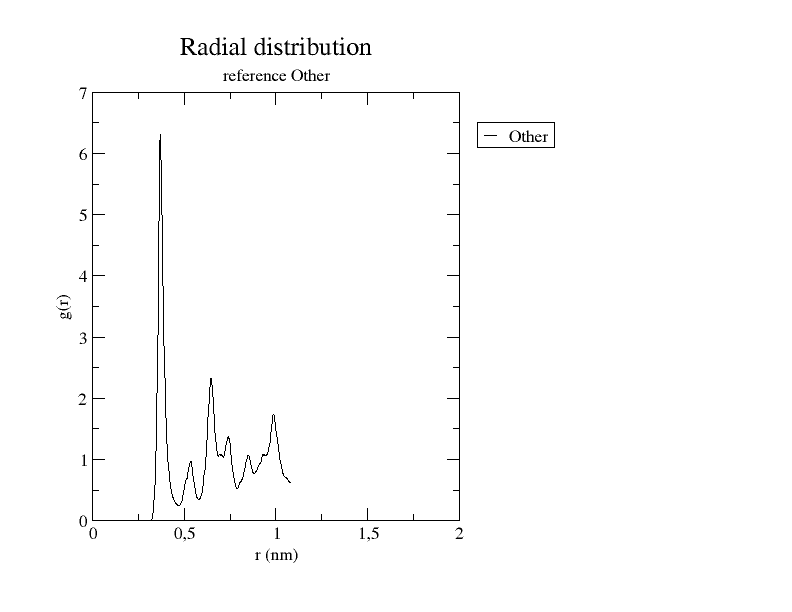
\includegraphics[width=180px]{plots/rdf_solid.png}
	\caption{Figure rdf from solid argon; correlation function against distance}
	\label{rdf solid}
\end{figure}

\begin{figure}[t]
	\centering
	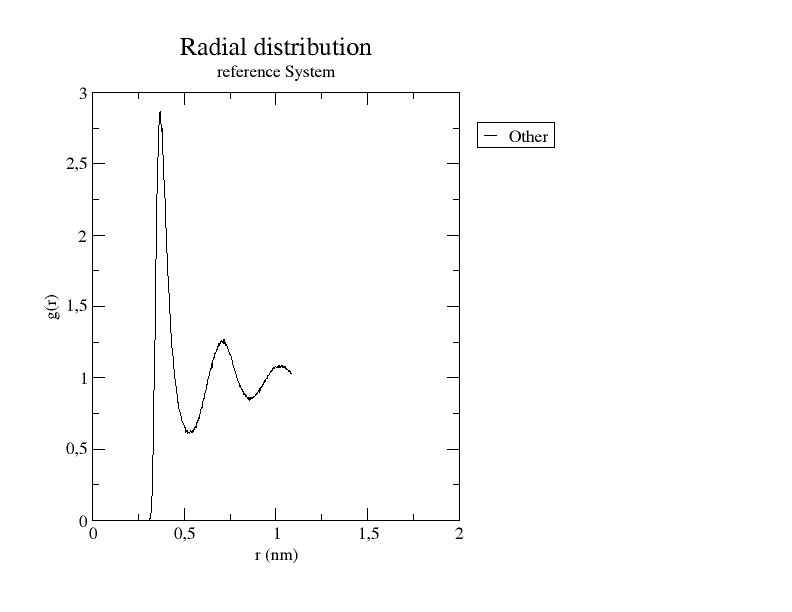
\includegraphics[width=180px]{plots/rdf_liquid.png}
	\caption{Figure rdf from solid argon; correlation function against distance}
	\label{rdf liquid}
\end{figure}

At both rdf before 0.3 there is zero correlation. The first peak is at r=0.37nm and g(r)=2.85 for liquid argon und g(r)=6.30 for solid argon, these are the highest peaks for each plot. In the liquid plot the next peak at 0.71nm. In the rdf plot for solid argon there is a small peak at r=0.54 with g(r) = 0.97 and a higher peak with g(r)=2.23 at r=0.65.

g(r) corrolation function, relation from bulk density(=average density) to local density(density from one molecule to an other) discribes the variation in density as a function of distance, so higher g(r) means more molecules at r.

Nearing r<3 the rdf is 0 as well for both states. This can be explained by the Lennard-Jones-Potential, because of the repulsion no two molecules are at close distance. The most molecules are at r=0.37, corresponding to the minimun in the LJP and experimental findings [QUELLEN].
In solid state the peaks are higher and well defined, because the atoms are densly packed. The second (high > 0) peak appears at r=0.65 wich is roughly twice the distance from the center. This shows the constant structure of the solid phase. The broadening of the shape is because of vibrating of the molecules.In comparison the rdf of liquid argon shows the first peak ate the same r, but g(r) is half the size, which means less atoms at this given distance. The second peak is not at twice the distance as the first. Liquids are moore loosely packed so the intervals aren't as exact as in solids.

%http://www.sklogwiki.org/SklogWiki/index.php/Argon
%https://www.ncbi.nlm.nih.gov/pmc/articles/PMC349093/?page=4

\begin{figure}[t]
    \centering
    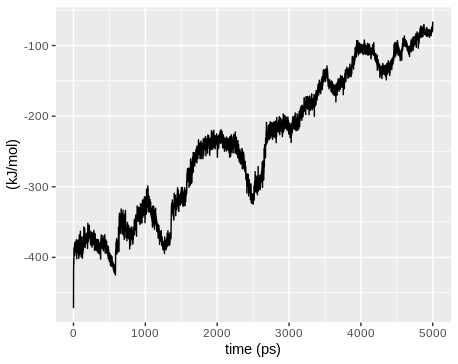
\includegraphics[width=180px]{plots/Heatup/pot_energy_heatup.png}
    \caption{x-axis: time in picoseconds; y-axis: potential energy in kilojoule; By increasing the tempreature of the system, the potential energy is rising. The thermostat fixes the kinetic energy, which can lead to a loss of potential energy (which can be seen in this plot). Particles can be accelerated or slowed down by the thermostat.}
    \label{heatup_potentialenergy}
\end{figure}

\begin{figure}[t]
    \centering
    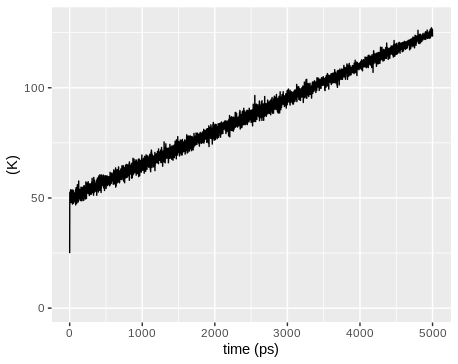
\includegraphics[width=180px]{plots/Heatup/temp_heatup.png}
    \caption{x-axis: time in picoseconds; y-axis: temperature in Kelvin; Heating of the system increases the overall temperature over time.}
    \label{heatup_tempreature}
\end{figure}

\begin{figure}[t]
    \centering
    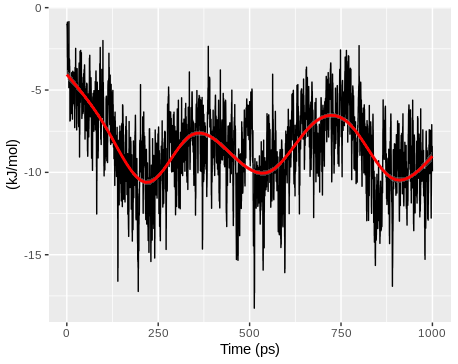
\includegraphics[width=180px]{plots/potential_energy.png}
    \caption{x-axis: time in picoseconds; y-axis: potential energy in kilojoule per mol; As we slowly decrease the temperature the system is losing kinetic energy. Due to the decrease of energy in the system, the potential energy also decreases.
The potential energy of atoms at higher temperatures is stored by electrons in excited states, additionally at higher temperatures more atoms are in excited rotationally states. ~\cite{chemguide}
Also the virial theorem specifies, that the potential energy and the kinetic energy in a system are depend on each other. ~\cite{cosmos-indirekt}}
    \label{gas_to_liquid_potentialenergy}
\end{figure}

\begin{figure}[t]
    \centering
    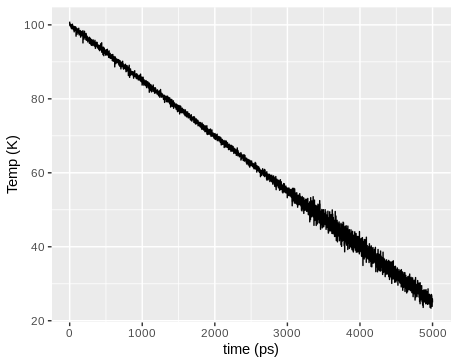
\includegraphics[width=180px]{plots/temp_plot.png}
    \caption{x-axis: time in picoseconds; y-axis: temperature in Kelvin; The cooling of the system reduces the overall temperature.}
    \label{gas_to_liquid_temperature}
\end{figure}

\begin{figure}[t]
    \centering
    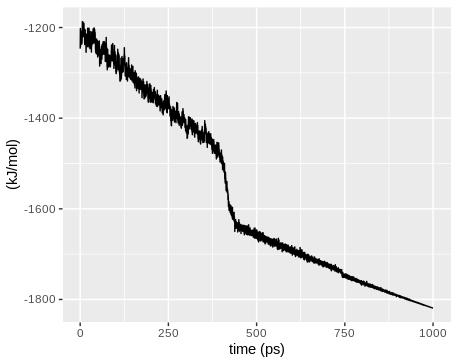
\includegraphics[width=180px]{plots//freezing/freezing_pot_en.png}
    \caption{x-axis: time in picoseconds; y-axis: potential energy in kilojoule; The decrease of temperature controled by the thermostat leads to a decreased potential energy.}
    \label{freezing_pot_en}
\end{figure}

\begin{figure}[t]
    \centering
    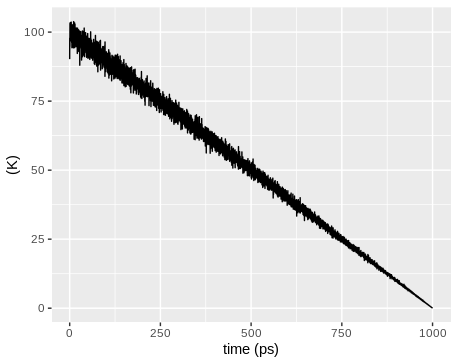
\includegraphics[width=180px]{plots//freezing/freezing_temp.png}
    \caption{x-axis: time in picoseconds; y-axis: temperature in Kelvin; The cooling of the system reduces the overall temperature.}
    \label{freezing_temp}
\end{figure}


\begin{thebibliography}{100}
\bibitem{Gonzalez} M.A.González: Force fields and molecular dynamics simulations. \textit{JDN}, Volume 12, 2011. 169 - 200. 2011.
\bibitem{Quant} P. A. M. Dirac: On the Theory of Quantum Mechanics, \textit{Proceedings of the Royal Society of London}, Series A 112, pp. 661—677. 1926.
\bibitem{Molekular} London, F.: Zur Theorie und Systematik der Molekularkräfte. 1930. 
\bibitem{chemguide}  \hyperlink{http://www.chemguide.co.uk/analysis/uvvisible/theory.html}{UV-visible absorption spectra [chemguide.co.uk]} (Zugegriffen am 21.03.2019 um 15:20 Uhr).
\bibitem{cosmos-indirekt} \hyperlink{https://physik.cosmos-indirekt.de/Physik-Schule/Virialsatz}{Virialsatz [physik.comsoms-indirekt.de]} (Zugegriffen am 21.03.2019 um 15:30 Uhr)
\end{thebibliography}

\end{document}


